\documentclass[reprint, nobibnotes, amssymb, amsmath, amsfonts, physics, mathtools, mathrsfs, floatfix]{revtex4-1}
\usepackage{graphicx}
\usepackage[english]{babel}

\newcommand{\redchi}{$\tilde{\chi}^2\,$}

\begin{document}

  \title{Relativistic Dispersion of Free Electrons}

  \author{Aman LaChapelle}
  \affiliation{The University of Chicago}

  \begin{abstract}
    We demonstrate the Hall Effect in a Germanium sample that is p-type doped with Gallium.  We observe hole conduction at low temperatures and measure a Hall coefficient of $(8.3 \pm 0.2)e+4\,C^{-1}$.  We further measure a resistivity in the direction of applied current of $2.59\pm0.09\,\Omega \cdot cm$  We measure an energy gap between valence and conduction bands in $Ge_{1-x}Ga_x$ of $0.64\pm0.06 \, eV$, and we measure $x = (1.70\pm0.05)e-9$.
  \end{abstract}

  \maketitle
  \tableofcontents

  \section{Introduction and Theory}
    The Hall effect is an effect that occurs when we run a current through a region with a perpendicular magnetic field.  The classical picture is that the electrons which move in cyclotron orbits in the bulk will move in a skipping motion at the edge and create edge currents, significantly, a current that induces a voltage difference that is perpendicular to the applied current/voltage.  This effect was famously first noticed by Edwin Hall in 1879~\cite{classical_hall}.  Later on, after the formalism proposed by Landau and Lifschitz ~\cite{landau}, and the nearly concurrent discovery by Von Klitzing of the exact quantization of the Hall conductivity~\cite{Von_Klitzing} did the solid state physics community begin to understand the quantum effects behind the Hall effect.

    Shortly after the discovery of the Integer Quantum Hall Effect (IQHE), came the discovery of what is now called the Fractional Quantum Hall Effect (FQHE).  The first observation of the FQHE was by Horst St\"{o}rmer and Dan Tsui~\cite{stormer_tsui}, searching for the theorized Wigner crystal that would form from electrons in a solid under extremely high mangetic fields.  Just a year later Robert Laughlin introduced the Laughlin wave function that did an excellent job of explaining this effect - now understood to be because of fractional filling of the landau levels.

    Subsequent discoveries in the realm of quantum Hall physics have mostly focused on topological nontriviality, and a current prevailing explanation uses Chern-Simons field theory to perform a singular gauge transformation in order to attach flux quanta to electrons in the form of vortices - a.k.a. zeros of the wave function.  We can think of the effect in a very simplistic way as electrons and vortices bound together in such a way that the electron wave function picks up a phase of $2\pi$ times the number of vortices that the electron is pinned to as it goes around.  This is (again very simplistically) an extension of the Aharonov-Bohm effect, and is beginning to be understood in terms of topological nontrivialities that are properties of the quantum system itself - another interpretation being the relation of the Berry phase to the Chern number of the system and characterizing its topological invariance.  It is important to recognize that much of this characterization occurs in real-space, which allows real-space measurements of system invariants such as the Chern number and other topological invariants.

    For our case, the classical theory provides enough formalism, as we are not dealing with a temperature, experimental resolution, or field at which partial filling factors come into play, we are only concerned with the voltage difference induced perpendicular to the induced voltage at a very classical level.  The essence of the Hall effect remains much the same - we will notice that the cause of the Hall voltage is still due to the landau quantization (however at high filling factors/currents it is nearly continuous) and the edge states that arise as a result of this quantization.  We can, however, describe much of this formalism in the classical limit with Dr\"{u}de theory as follows.

    If we consider electrons/holes as simple masses traveling through a region with a certain net velocity (drift velocity) and time between scattering events (mean free time), where the current is described by
    \begin{equation}
      j = -nev_d
    \end{equation}
    we can then define a conductivity tensor and simply write down the Lorentz force equation to return the Hall Voltage and Resistance as the following:
    \begin{gather}
      R_H = \frac{1}{q n} = \frac{E_y}{j_x B_z} \label{hall_resist} \\
      V_H = R_H j_x B_z w \label{hall_volt}
    \end{gather}
    with $j_x$ the applied current and w the width of the sample.  It is important to note that we have defined the Hall Resistance in terms of the charge, $q$, when it is normally defined in terms of the electron charge, $-e$, or the hole charge, $+e$, depending on the primary charge carrier.

    Now, with a basic understanding of band theory, we can rewrite this a little in order to take better accounting of electrons and holes and potentially different scattering characteristics.  We rewrite the current (and the drift velocity) in terms of the mobility and get the following equations that allow us to take into account different charge carriers in different systems:
    \begin{gather}
      \mu_{h/e} = \frac{e \tau_e/h}{m_{e/h}^*} \label{mobility} \\
      \text{Which leads us to the following:} \nonumber \\
      \sigma = e(n_h\mu_h + n_e\mu_e) \label{conductivity} \\
      \rho = \frac{1}{e(n_h\mu_h + n_e\mu_e)} \label{resistivity} \\
      R_H = \frac{E_y}{j_x B_z} = \frac{\mu_h^2 n_h - \mu_e^2 n_e}{\sigma^2/e} \label{rh_mob_sigma}
    \end{gather}
    with $\sigma$ being the conductivity we are familiar with from Ohm's law.  Note that $n_{h/e}$ are the concentrations of holes and electrons, respectively and $\mu_{h/e}$ are the mobilities of the same.  $m_{e/h}^*$ is the band effective mass of an electron or hole respectively.  This formulation suggests the definition of a new quantity, the Hall mobility:
    \begin{equation}
      \mu_H = |R_H|\sigma \label{hall_mobility}
    \end{equation}
    which allows us to relate resistivity of a given semiconductor in and out of a magnetic field in a phenomenon known as magnetoresistance - which is the same phenomenon wherein we see peaks of resistivity at the quantized Hall plateaus - the resistance in the induced direction increases sharply as we come to quantized values for the Hall resistance.

    There are two types of dopants for semiconductors - p-type and n-type.  n-type semiconductors donate negative charges, or electrons, to the semiconductor band structure, resulting in the main charge carrier being an electron that can move freely throughout the bulk.  P-type dopants accept electrons, creating holes in the band structure which still allows for charge flow but now holes are the dominant charge carrier.  This becomes manifestly true at low temperatures especially due to the fact that at low temperatures the electrons bound to the bulk atoms are stuck, and the only things moving will be the dopant particles (or quasiparticles as is the case with holes).

    Semiconductors have an intrinsic resistance called magnetoresistance when they are placed in a magnetic field.  Luckily, we can correct for this quite simply, and we will simply state what we use pushing forward to understand and correct for this effect.

    \begin{equation}
      \rho_B = \rho_0(1 + \mu_H^2 B^2) \label{magnetoresistance}
    \end{equation}

    \section{Experimental Methods}
    In order to measure the Hall voltage and from that the resistivity and the Hall coefficient, we made the following electrical measurements.  If we refer to Figure~\ref{circuit_diagram}, we notice that we run current through the sample in the direction from point 5 to point 6.  We can then directly measure the Hall voltage by measuring the difference between ports 1 and 2, or 3 and 4.  Now, it is possible that these ports are not perfectly horizontal with each other - that is, they might not be normal to both the current propagation \textbf{and} the magnetic field, and so we will take data by making rotations - henceforth referred to as '+' and '-'.  The idea is that if we take data at one orientation and then at the other, we will be able to simply average out the effect from the offset of the measurement ports.  From the data that we collect, we are able to directly calculate values for $R_H$, $\mu_h$ and $\rho$.  From these there are other values we can derive such as the magnetoresistance and density of charge carriers (holes).

    In order to take data as a function of temperature, we raised the temperature by running current through a 130$\Omega$ resistor in small increments, and then taking a scan first at the '+' orientation and then at the '-' orientation.  We repeat this 75 times in the temperature interval between 86 K and 374.9 K.  The goal is to perform this measurement between 77 and 375, but due to the fact that in opening the cryostat to remove the $LN_2$, the copper - and thus the sample - warmed up considerably - a full 9K.

    As we heat up to room temperature it takes more to heat up the sample, and as we go above room temperature the data has to be taken carefully as the sample tends to cool rather than warm up more once it settles.  Care must be taken through the whole range to ensure the temperature of the scans between the '+' and '-' orientations are as close as possible, but as long as we are cautious and wait long enough so the temperature fluctuations are kept low the maximum variation can be kept to less than 0.5K, in many cases we measured differences of between 0.1 and 0.2 K between the '+' and '-' orientations.

    \section{Analysis}
    The first measurements that we made were at 77K, the approximate temperature of $LN_2$.  We first set out to measure the number concentration of Gallium dopants (and through that the concentration of charge carriers), as well as the hole mobility.  First, however, we must measure the Hall voltage and from that extract the Hall coefficient, $R_H$.  The values we measured are summarized in Table~\ref{tab:results}.  The first thing to notice is that our concentration of Gallium atoms is very close to what others have reported for the same sample, so this gives us some confidence that going forward, our data will at least make sense.  If we then calculate, using the density of Germanium, the ratio of Gallium to Germainum atoms, we see that the ratio is $(1.70\pm0.05)e-9$, which makes sense for a mild dopant.  It's not large, but it's enough to provide some mild p-type doping for conductivity at low temperatures, where $k_B T$ isn't usually large enough to excite an electron into the valence band.

    The next thing we will notice is that we have calculated two values for the hole mobility, again if we look at Table~\ref{tab:results}.  We notice that the result that we calculate from equation~\ref{hall_mobility} is smaller than the result we calculate from equation~\ref{magnetoresistance}, and has a larger uncertainty.  This is because when we removed the sample from the B field one of the wires shorted or something similar - the voltage across those leads suddenly dropped to close to zero - and we were unable to make use of the 2 and 4 connections and average with the 1 and 3 values as we were able to for the magnetoresistance value (specifically, $\rho_B$) which increased our uncertainty - perhaps not to the level that this exhibits, but still did increase it.  This is not optimal, and had we noticed earlier we would have corrected it but sadly we did not notice until the lab was over.  Luckily, we still do have data that we can use and that is still admissable, and we will simply use this data for the remainder.  Furthermore, the two values are still within uncertainties of each other, and both are slightly less than the given value of $48000 \,  \frac{cm^2}{V\cdot s}$, not significantly less which is what we would expect for a sample that is doped as mildly as this one is.

    If we assume that the carrier concentration is fixed and the mobility is the only thing that changes with temperature, we can write down what we expect for $R_H$ and $\rho$.  We expect that $R_H$ is constant as we can see in equation~\ref{hall_resist} (with q = e), while we expect that $\rho$ is increasing with temperature as we can see from equation~\ref{resistivity} (with $n_e = 0$).  We can actually observe these effects if we look at figures~\ref{RH_vs_T} and~\ref{rho_vs_T}.  We notice that the Hall coefficient is increasing until about 250K-275K, at which point it decreases rapidly.  This is due to the fact that in this region the hole mobility decreases very quickly and the electron mobility begins to increase.  We can see this from equation~\ref{rh_mob_sigma}, where as we increase the temperature the electron (as carriers) density increases to a point and thus the numerator decreases. Furthermore we know that the mobility has some temperature dependence, thus it stands to reason that this would be the explanation for the phenomenon.  Also possible is that the density of electrons as charge carriers is simply increasing greatly, which would cause the same effect.  We could test which one it is by choosing a non-doped sample and performing the same experiment to find out what the electron mobility does as a function of temperature, or we could use an n-doped sample and doing the same.  Either way, the goal is to test the electron mobility and density rather than hole mobility and density as we are doing here.

    The other thing that we notice is that at the high temperature extreme, we notice that the Hall coefficient goes to zero.  This is to be expected - at high temperatures we would expect electrons to be flying all over the place, and we would thus expect the Hall coefficient to tend to zero at high temperatures as it clearly does here.  This is nothing new, however, the interesting point is where it falls rapidly to below zero and then comes back up to zero.  The temperature at which $R_H$ hits zero is at $325\pm1$ K.  We determine this by taking the points closest to the zero point and averaging between them~\ref{RH_vs_T} (the equivalent to fitting a line between them and plugging in for zero that way).  We get an equivalent result from taking our fitted form for $R_H$ and solving for the $R_H = 0$ intercept.  In order to perform this fit, we have taken the single point above $R_H = 0$ and the points below 0, and fit to the following form:
    \begin{equation}
      -Ae^{\frac{E_g}{2 k_B T}} + \frac{B}{(T-C)^2}
    \end{equation}
    where the second term accounts for the things that happen before we reach temperatures at which the mobilities are no longer temperature dependent.  We expect
    \begin{equation}
      R_H = \frac{-(\mu_e^2 - \mu_h)^2}{en_e(\mu_e + \mu_h)^2}
    \end{equation}
    and at high temperatures we want
    \begin{equation}
      R_H = -Ae^{\frac{E_g}{2 k_B T}}
    \end{equation}
    so in the middle, where $R_H$ is just crossing zero, we would expect to have some mixture of the two.  Since we do not know the exact temperature dependence of the mobilities, but we do know some basic physics about mobilites, we expect this $1/T^2$ term.  This is because we do not expect the mobilities to diverge to positive and negative infinity at any value, if they do diverge we expect it to be to positive infinity only.  We do not expect it to go to infinity, but we also cannot (for the sake of time) fit this to half a lorentzian, so we have fit to this form as it models the behavior we see here and approximates a lorentzian in this limit where we only care about one tail and the top might as well go to infinity.

    We can see the results of this fit in figures~\ref{rh_12_eg} and~\ref{rh_34_eg}.  We fit the two Hall coefficients separately in order to perform a sort of double-blind experiment, and make sure that we can be confident in our extracted values of the gap energy.  We notice that the extracted values are certainly within uncertainties of each other, and are within uncertainties of the accepted value of 0.67 eV.  This may present false security however, because it is possible that the higher-temperature region of the fit is distorting the portion that is fit to the expected form (just the exponential part).  However, we believe that the strategy we have employed is also valid and results in a more accurate determination of $E_g$ because it relies less on picking data points that fit the model.  If we do pick the data points, we only end up using the last 8 points in the dataset and the fit is very subpar.  We find from a fit like that (not shown) a value for $E_g = 0.7 \pm 0.1$ eV because there are so few points and the simulations returned a massive standard deviation in the fit values.  Furthermore, the $\chi^2$ value was tiny, on the order of 0.01, which indicates that we were overfitting and so that fit was scrapped.

    We propagated fractional uncertainties and then multiplied those values by the values of $R_H$.  Since the values of $R_H$ are quite large, even a fractional uncertainty of 1\% or less (in this case it's about 0.3\%) can show up as quite large towards the higher end of the scale, but not here.

    In order to determine the uncertainties in the value of $E_g$ we simulated random datasets using a normal distribution - we picked points at random from within the uncertainty of each actual point and fit those datasets - from this we find the standard deviation of the fitted energies (fits performed on simulated data) and take that to be the uncertainty.  This technique was also performed on the fit that we presently shift attention to, the fit of resistivity and temperature to find the same gap energy.

    The fit shown in figure~\ref{rho_eg}, where we fit the resistivity as a function of temperature, exhibits a different gap energy, one which is not within uncertainties of the accepted value nor is it within uncertainty of the other values we found.  This is due to many things, most likely because this quantity is temperature dependent which causes distortion of the effect if we are using points above 300K (we are using points at 325K-375K in this fit).  It is also likely due to the fact that we are only using the tail end of the resistivity, and would likely get a better result if we were to fit more of the resistivity.  This, however, is quite difficult and time consuming, so we must be satisfied with the results we have.

    \section{Conclusion and Tables \& Figures}
    If we take a look at Table~\ref{tab:eg}, we see that some of our values are within uncertainties of the accepted value and the other is not.  We have already discussed reasons for why this is likely the case, but it is also possible that this is an extension of a systematic uncertainty that applies broadly across the whole lab.

    All our temperature measurements depended on the fact that there was a reference in ice water.  Though we did check and the water was still icy throughout the lab, it is possible that the temperature changed slightly.  Furthermore, in taking data, when we switched the orientation and then repeated the scan, there was perpetually a small difference in the temperature between the two orientations.  Together we estimate that these account for a total uncertainty on the temperature on the order of <1K, but it would systematically shift all of our data.

    Other uncertainties were propagated in quadrature - measurements in length and current are assumed to be independent, so, for example, in calculating the uncertainty in the Hall coefficient we used the following:
    \begin{equation}
      \frac{\delta R_H}{R_H} = \sqrt{ \left(\frac{\delta V_H}{V_H}\right)^2 + \left(\frac{\delta t}{t}\right)^2 + \left(\frac{\delta I}{I}\right)^2 + \left(\frac{\delta B}{B}\right)^2 }
    \end{equation}
    with $t$ being the thickness, $B$ being the magnitude of the measured magnetic field, and $I$ being the current readout on the apparatus.  In measuring the magnetic field, we used a gaussmeter that was calibrated and, as with all gaussmeters, had a fairly accurate readout, but was not perfect.  It tended to fluctuate by up to 60G, which we accounted for, but it is possible that the calibration was off and we simply did not notice, and that could have caused an additional fractional uncertainty of up to 5\% in B, which would have caused systematic errors propagated through of up to 3\% in any given value - almost all of them made use of $B$ and its uncertainty.  Luckily, this is quite small, and doesn't push any of our measured values far away from the accepted values, and possibly even helps us to push the value we recovered from the resistivity into the range of the accepted value.  Note that this is speculation, as we are not sure about any of these sources of systematic uncertainty, but if we take all of the mentioned sources of systematic uncertainty ($T$, $B$) into account by shifting temperatures down by 0.7K and increasing the uncertainty in $\rho$ by 3\%, we see in the value of $E_g$ that we get a value of $0.75\pm0.03$ eV, not a huge shift and still not within uncertainties of the accepted value, but it does suggest that something like a systematic uncertainty is causing our value to be different from the accepted value.

    We would like to thank all the staff of the Advanced Undergraduate Physics Laboratory, and especially Will Foreman for putting up with questions that we should have addressed much earlier and patiently helping and dealing with our impatience.

    \subsection{Tables}

    \begin{table}[h]
      \begin{tabular}{|c|c|c|}
        \hline
        Quantity & Value & Uncertainty \\ \hline
        $V_H$ & 0.02463 $V$ & 0.00004 \\ \hline
        $R_H$ & 83000 $C^{-1}$ & 2000 \\ \hline
        $N_A$ &  7.5e+13 $cm^{-3}$ & 2e+12 \\ \hline
        $\rho_B$ & 2.6 $\Omega \cdot cm$ & 0.1 \\ \hline
        $\rho_0$ & 2.3 $\Omega \cdot cm$ & 0.1 \\ \hline
        $\mu_h$, Eq.~\ref{hall_mobility} & 37200 $\frac{cm^2}{V\cdot s}$ & 7500 \\ \hline
        $\mu_h$, Eq.~\ref{magnetoresistance} & 40000 $\frac{cm^2}{V\cdot s}$ & 2000 \\ \hline
      \end{tabular}
      \caption{A summary of important results.~\label{tab:results}}
    \end{table}

    \begin{table}[h]
      \begin{tabular}{|c|c|c|}
        \hline
        $E_g$ from: & Value (eV) & Uncertainty (eV) \\ \hline
        Accepted & 0.67 & negligible \\ \hline
        $R_{H, 12}$ & 0.64 & 0.06 \\ \hline
        $R_{H, 34}$ & 0.64 & 0.06 \\ \hline
        $\rho$ & 0.76 & 0.01 \\ \hline
      \end{tabular}
      \caption{Summary of the gap energies measured - we see that the gap energy that comes from the fitting of the resisitivity is off, likely from a distortion in the fit, or some other cause. \label{tab:eg}}
    \end{table}

    \hspace{.5cm}

    \subsection{Figures}

    \begin{widetext}

      \begin{figure}[h]
        \centering
        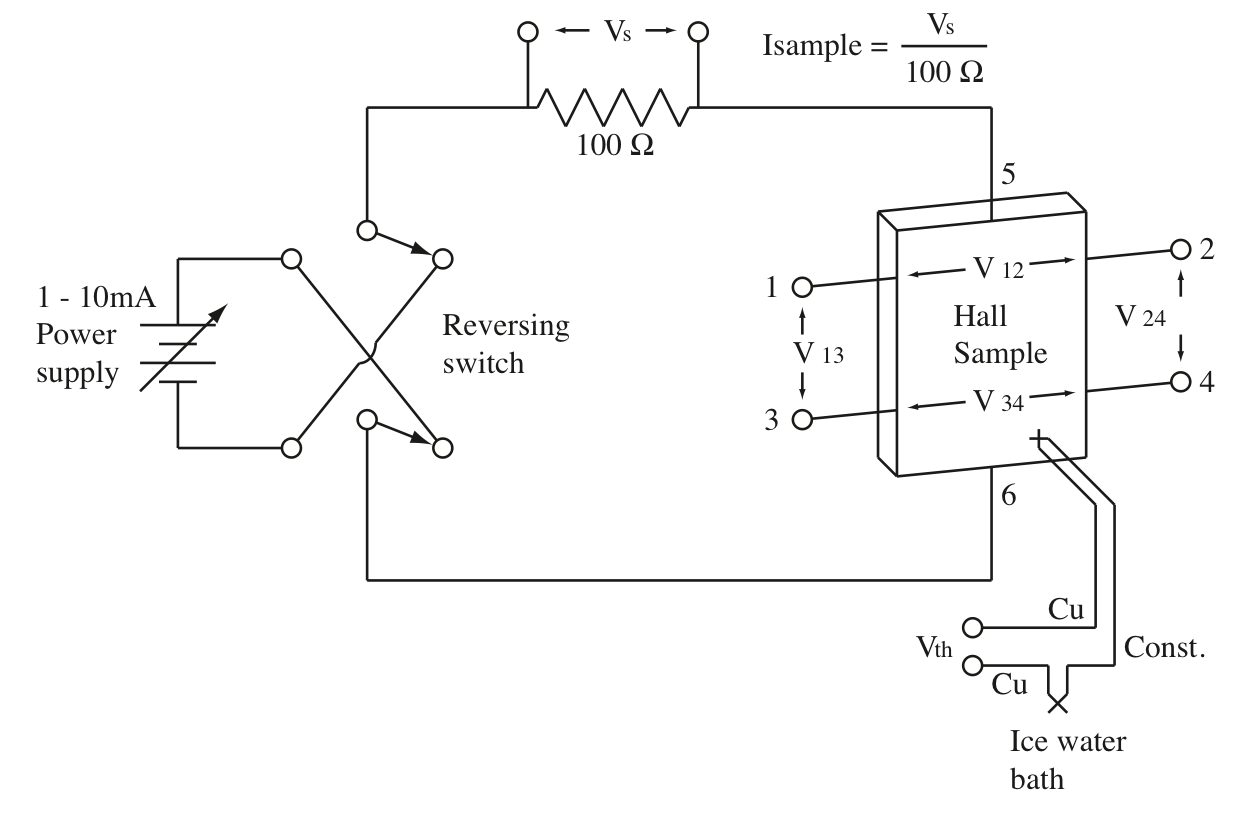
\includegraphics[width=\linewidth]{circuit_diagram.png}
        \caption{A wiring diagram for our experimental apparatus - this is illustrative in understanding the mechanics of the data collection process.~\label{circuit_diagram}~\cite{lab_manual}}
      \end{figure}

      \begin{figure}[h]
        \centering
        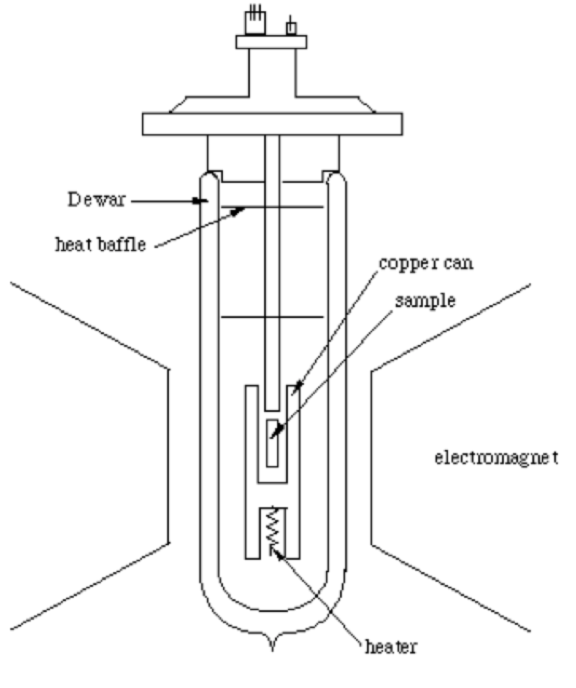
\includegraphics[width=\linewidth]{dewar.png}
        \caption{This shows the cryostat that held our GeGa sample.  The inside, as we can see, was glass to avoid heat conduction to the outer walls of the dewar.  The whole ensemble was placed between the poles of an electromagnet used to produce the strong $\vec{B}$ field that we needed in order to make measurements of our sample.  The whole apparatus turned through an angle of $2\pi$, with detents at $0$ and $\pi$ so that we could accurately take data at two rotations differing by almost exactly $\pi$ - we take uncertainties in this measurement to be less than 0.5 degrees because of the detente that could not move.  Furthermore, this uncertainty would be random and would not show up on every point, and even if we did account for it, we might see a change of less than 0.1\% in any given value.~\label{dewar}~\cite{lab_manual}}
      \end{figure}

      \begin{figure}[h]
        \centering
        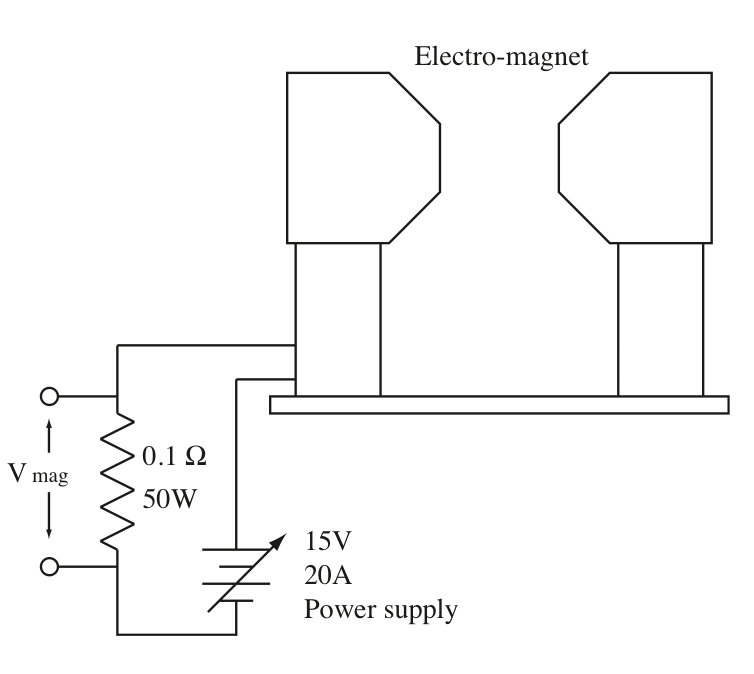
\includegraphics[width=\linewidth]{magnet_setup.png}
        \caption{We needed an extraordinarily strong magnet to see the Hall effect in action, thus we have a large solenoid with an iron core that directs the field generated by the 1000-turn electromagnet through the sample to achieve a field of $900\pm50$ Gauss at the center of the apparatus.~\label{magnet}~\cite{lab_manual}}
      \end{figure}

      \begin{figure}[h]
        \centering
        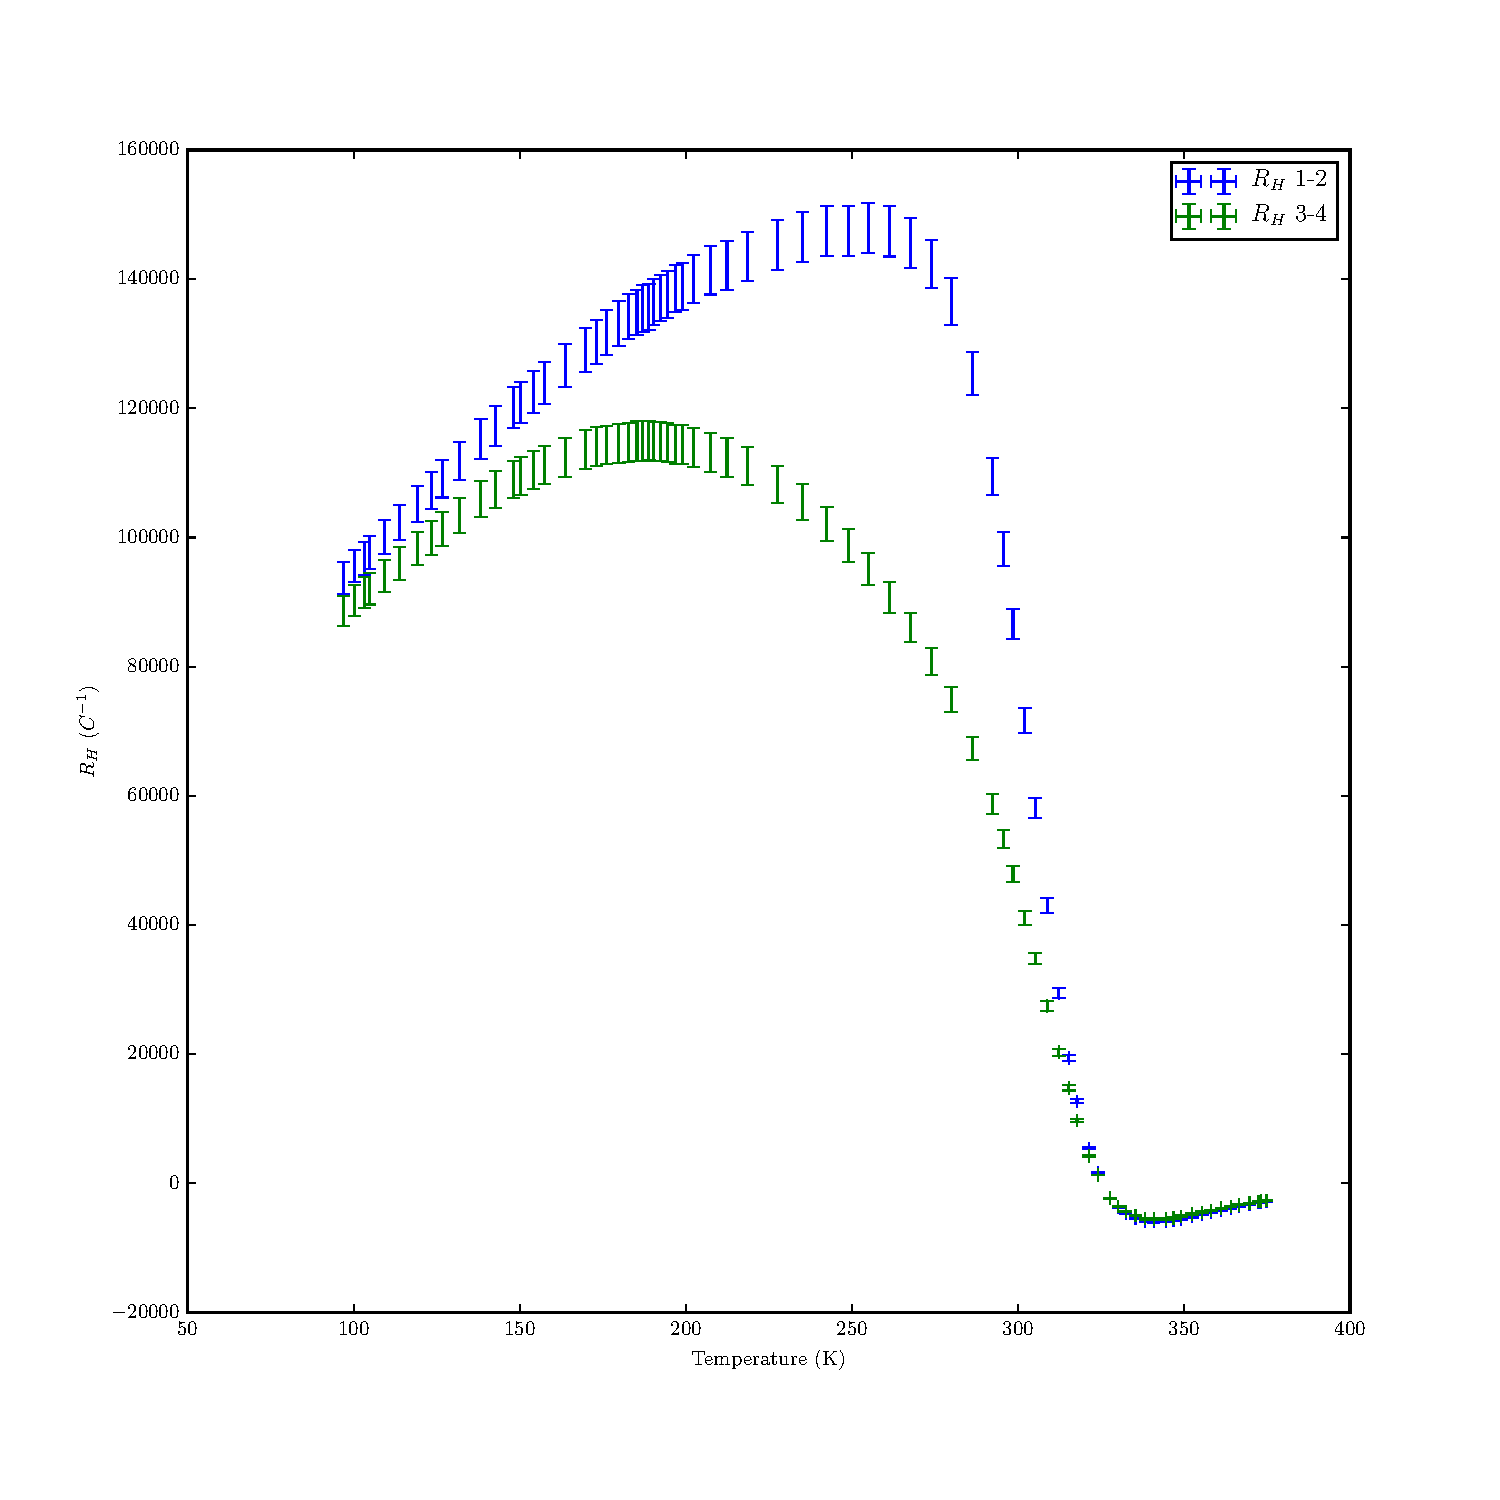
\includegraphics[width=\linewidth]{../plots/T_vs_R_H.pdf}
        \caption{Plotting the Hall coefficient as a function of temperature, the two traces are the two different leads - one dataset comes from leads 1 and 2, the other from 3 and 4, see figure~\ref{circuit_diagram} \label{RH_vs_T}}
      \end{figure}

      \begin{figure}[h]
        \centering
        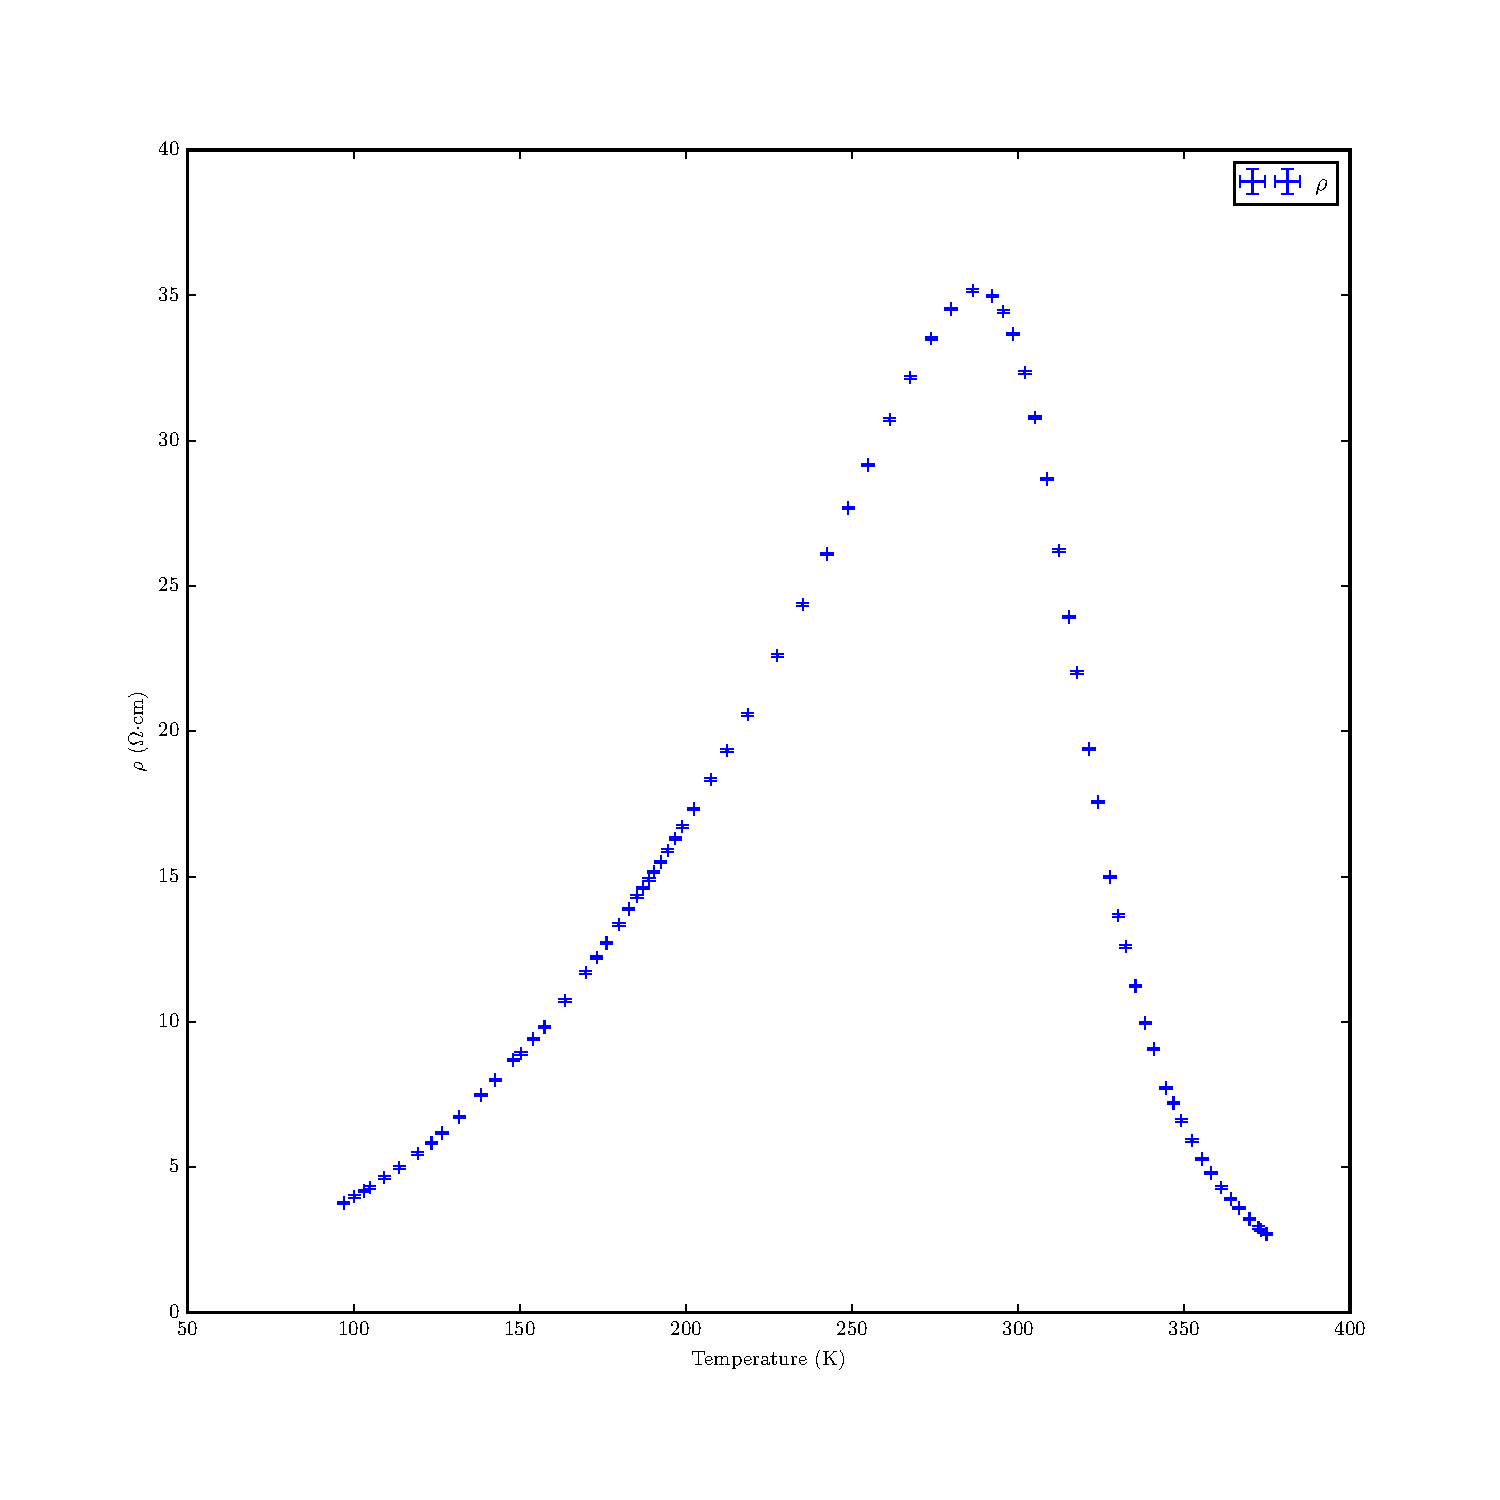
\includegraphics[width=\linewidth]{../plots/rho_vs_T.pdf}
        \caption{Plotting the resisitivity - from 5 to 6, see figure~\ref{circuit_diagram} \label{rho_vs_T}}
      \end{figure}

      \begin{figure}[h]
        \centering
        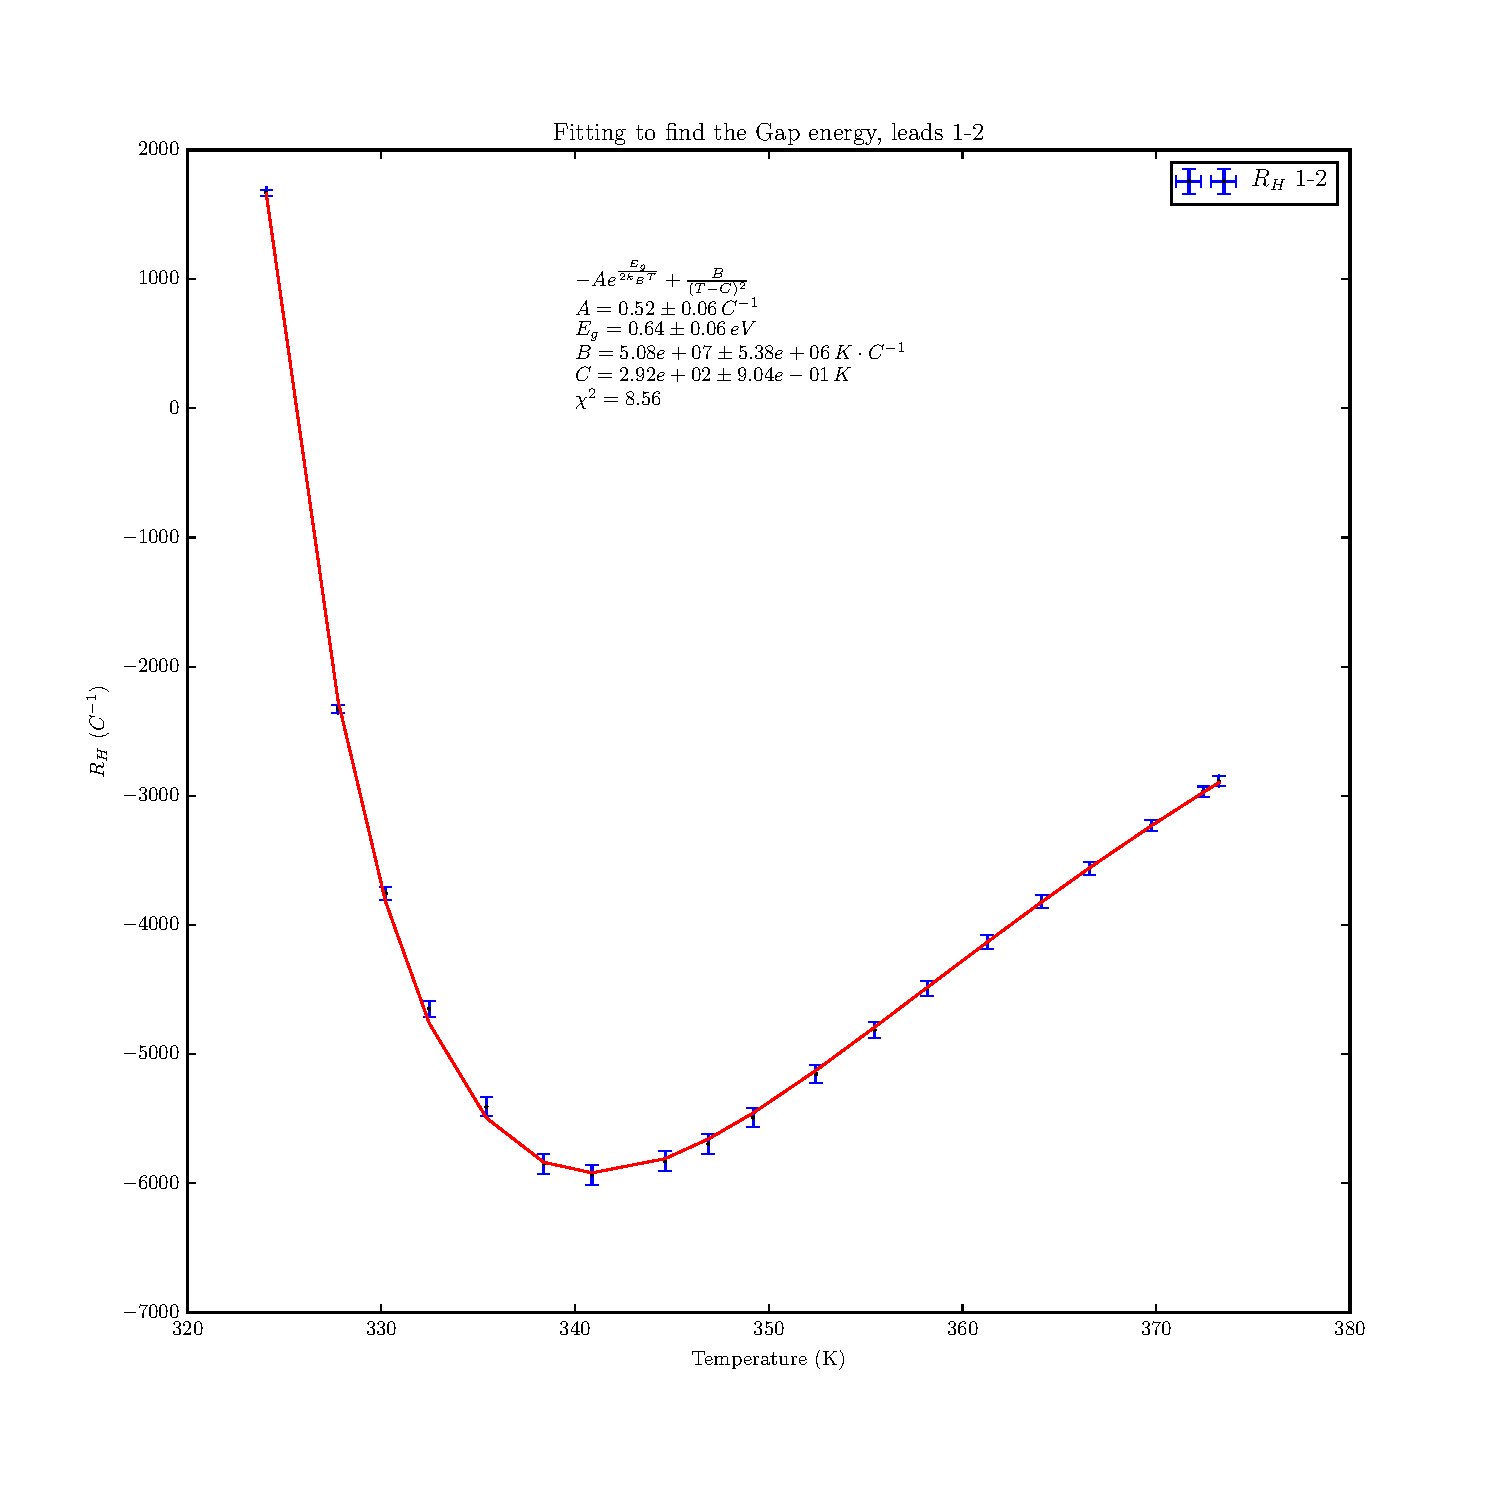
\includegraphics[width=\linewidth]{../plots/rh_12_eg.pdf}
        \caption{Fitting to find the gap energy for this particular sample.  We fit the Hall coefficient for $T > T_0 = 325$ for leads 1 and 2.  We had a \redchi value of 0.68, which indicates that we are either overfitting or we have overestimated our uncertainty in these points.  We believe that our uncertainty is correct, as we were not able to take more precise data, and the fit form works quite well, as we see in the fitting for the other hall coefficient and we can verify visually. \label{rh_12_eg}}
      \end{figure}

      \begin{figure}[h]
        \centering
        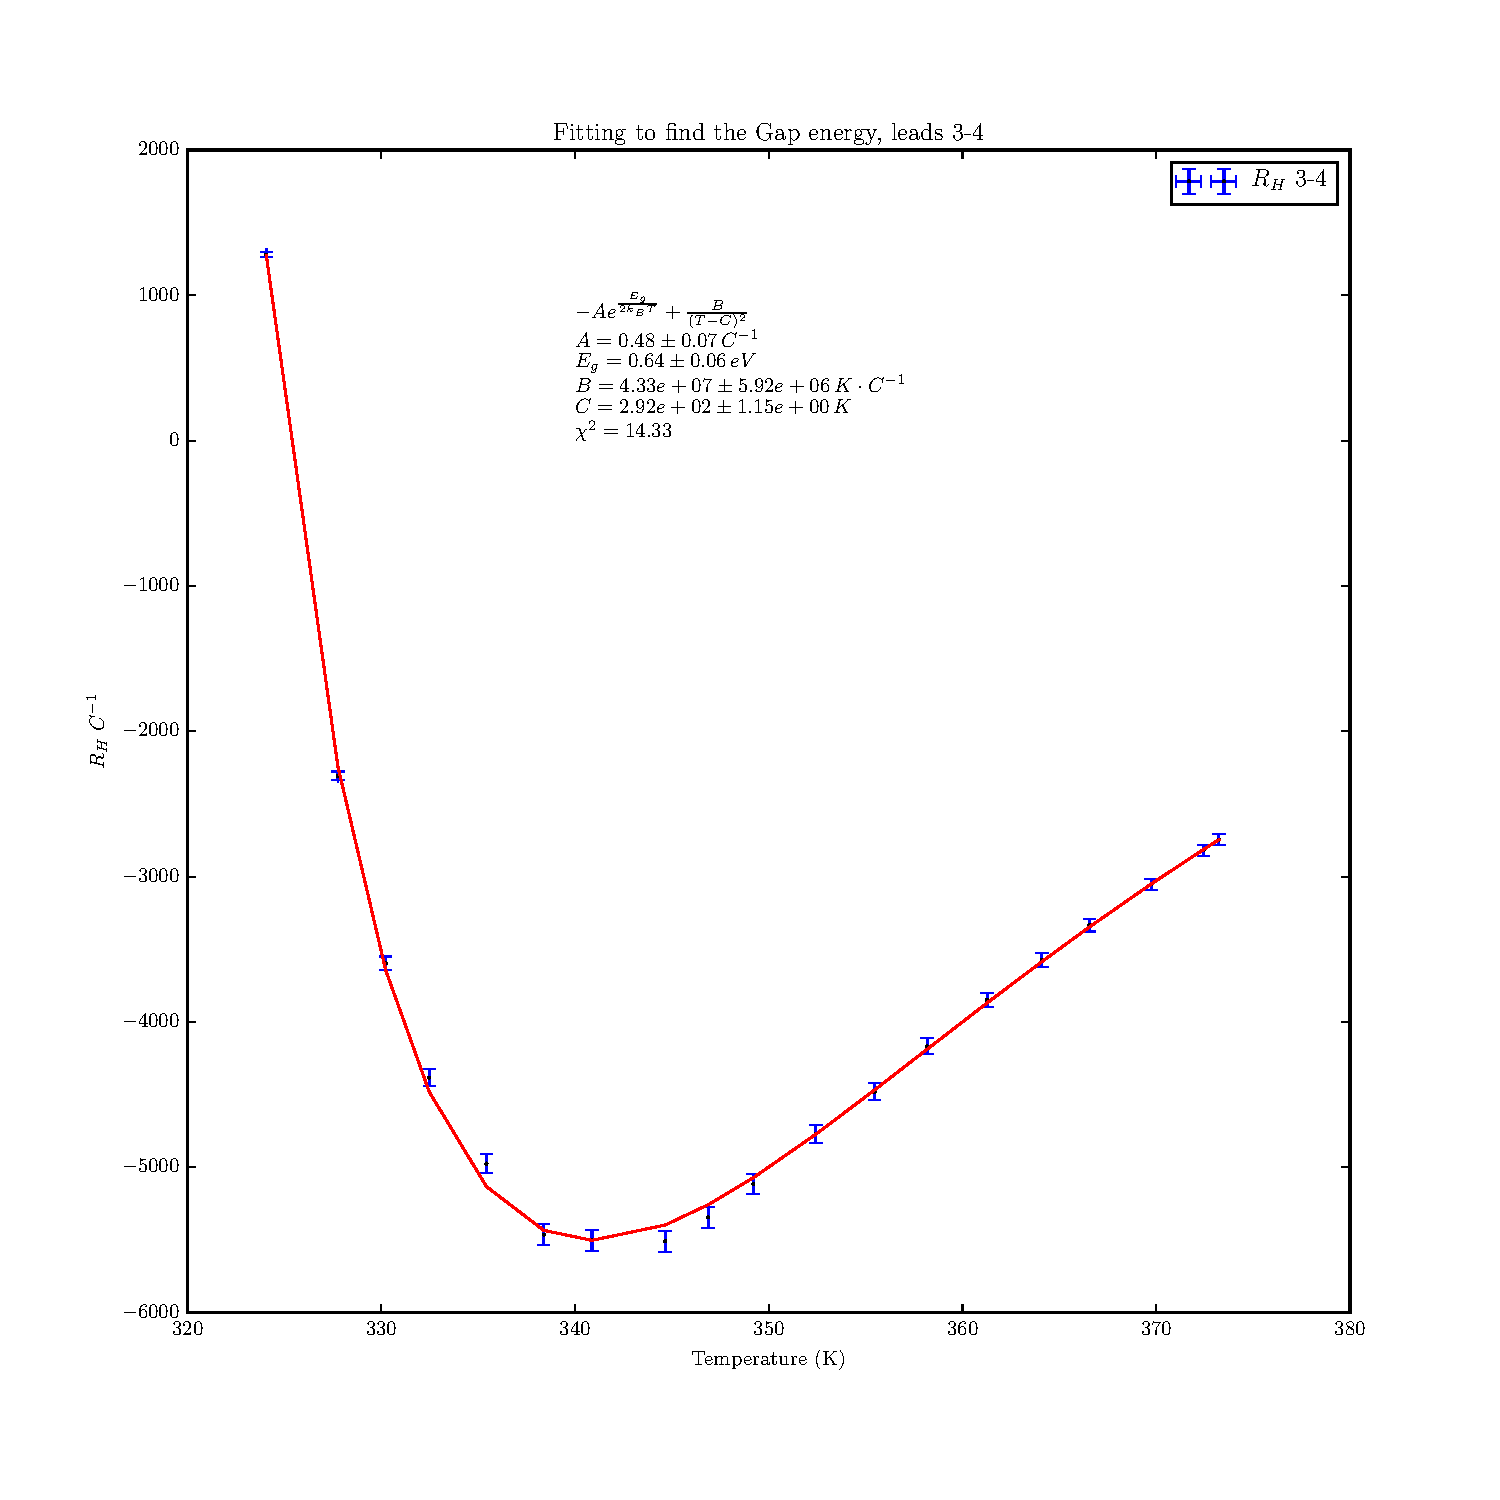
\includegraphics[width=\linewidth]{../plots/rh_34_eg.pdf}
        \caption{Fitting to find the gap energy for this particular sample.  We fit the Hall coefficient for $T > T_0 = 325$ for leads 3 and 4.  We had a \redchi value of 1 (0.977), which indicates an excellent fit. \label{rh_34_eg}}
      \end{figure}

      \begin{figure}[h]
        \centering
        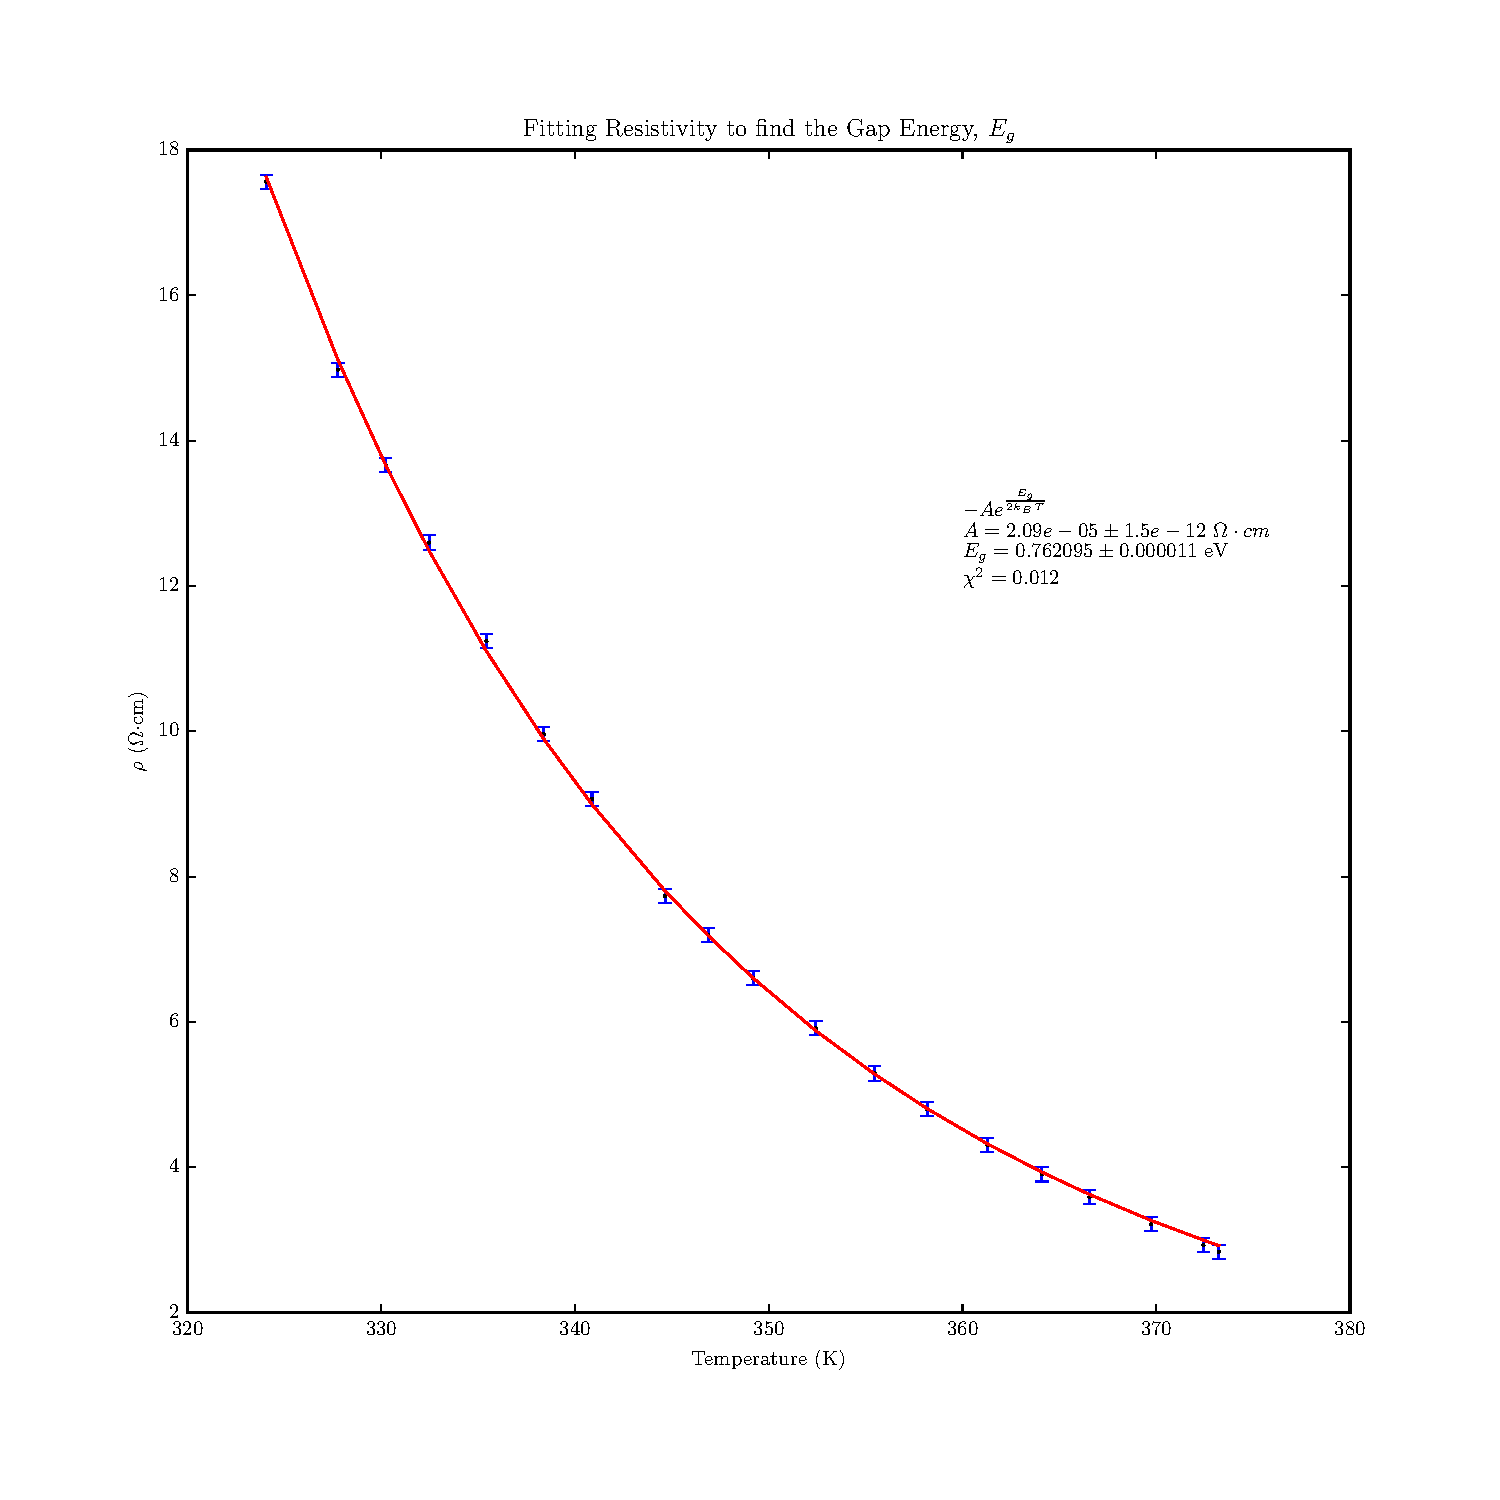
\includegraphics[width=\linewidth]{../plots/resistivity_eg.pdf}
        \caption{Fitting to find the gap energy for this particular sample.  We fit the resistivity (leads 5 and 6) for $T > T_0 = 325$. \label{rho_eg}}
      \end{figure}

    \end{widetext}

  \bibliography{bibliography}
  \bibliographystyle{plain}

\end{document}
